
%%%%%%%%%%%%%%%%%%%%%%%%%%%%%%%%%%%%%%%%%%%%%%%%%%%%%%%%%%%%%%%%%%%%%
%% This is a (brief) model paper using the achemso class
%% The document class accepts keyval options, which should include
%% the target journal and optionally the manuscript type.
%%%%%%%%%%%%%%%%%%%%%%%%%%%%%%%%%%%%%%%%%%%%%%%%%%%%%%%%%%%%%%%%%%%%%
\documentclass[manuscript=suppinfo]{achemso}

%%%%%%%%%%%%%%%%%%%%%%%%%%%%%%%%%%%%%%%%%%%%%%%%%%%%%%%%%%%%%%%%%%%%%
%% Place any additional packages needed here.  Only include packages
%% which are essential, to avoid problems later. Do NOT use any
%% packages which require e-TeX (for example etoolbox): the e-TeX
%% extensions are not currently available on the ACS conversion
%% servers.
%%%%%%%%%%%%%%%%%%%%%%%%%%%%%%%%%%%%%%%%%%%%%%%%%%%%%%%%%%%%%%%%%%%%%
% \usepackage[version=3]{mhchem} % Formula subscripts using \ce{}
\usepackage[T1]{fontenc}       % Use modern font encodings
\usepackage{graphicx,amsmath,mathrsfs}
\usepackage{xcolor}
\usepackage{todonotes}        % Remove on submission


%%%%%%%%%%%%%%%%%%%%%%%%%%%%%%%%%%%%%%%%%%%%%%%%%%%%%%%%%%%%%%%%%%%%%
%% If issues arise when submitting your manuscript, you may want to
%% un-comment the next line.  This provides information on the
%% version of every file you have used.
%%%%%%%%%%%%%%%%%%%%%%%%%%%%%%%%%%%%%%%%%%%%%%%%%%%%%%%%%%%%%%%%%%%%%
% \listfiles

%%%%%%%%%%%%%%%%%%%%%%%%%%%%%%%%%%%%%%%%%%%%%%%%%%%%%%%%%%%%%%%%%%%%%
%% Place any additional macros here.  Please use \newcommand* where
%% possible, and avoid layout-changing macros (which are not used
%% when typesetting).
%%%%%%%%%%%%%%%%%%%%%%%%%%%%%%%%%%%%%%%%%%%%%%%%%%%%%%%%%%%%%%%%%%%%%
\newcommand*\subs[1]{_{\text{#1}}} % Text subscription
\newcommand*\sups[1]{^{\text{#1}}} %Text superscription
\newcommand*\change[1]{\textcolor{cyan}{#1}}
\newcommand*\E[1]{\mathscr{E}\subs{#1}}
% \newcommand{\beginsupplement}{%
%         \setcounter{table}{0}
%         \renewcommand{\thetable}{S\arabic{table}}%
%         \setcounter{figure}{0}
%         \renewcommand{\thefigure}{S\arabic{figure}}%
%      }
%%%%%%%%%%%%%%%%%%%%%%%%%%%%%%%%%%%%%%%%%%%%%%%%%%%%%%%%%%%%%%%%%%%%%
%% Meta-data block
%% ---------------
%% Each author should be given as a separate \author command.
%%
%% Corresponding authors should have an e-mail given after the author
%% name as an \email command. Phone and fax numbers can be given
%% using \phone and \fax, respectively; this information is optional.
%%
%% The affiliation of authors is given after the authors; each
%% \affiliation command applies to all preceding authors not already
%% assigned an affiliation.
%%
%% The affiliation takes an option argument for the short name.  This
%% will typically be something like "University of Somewhere".
%%
%% The \altaffiliation macro should be used for new address, etc.
%% On the other hand, \alsoaffiliation is used on a per author basis
%% when authors are associated with multiple institutions.
%%%%%%%%%%%%%%%%%%%%%%%%%%%%%%%%%%%%%%%%%%%%%%%%%%%%%%%%%%%%%%%%%%%%%
\author{Tian Tian}
% \affiliation{Institute for Chemical and Bioengineering, ETH Z{\"u}rich,  Vladimir Prelog Weg 1, CH-8093 Z{\"u}rich, Switzerland}
\affiliation{Institute for Chemical and Bioengineering, ETH Z{\"u}rich, Z{\"u}rich 8093, Switzerland}

\author{Peter Rice}
\affiliation{School of Mathematics and Physics, Queen's University Belfast, United Kingdom}
\alsoaffiliation{School of Chemistry and Chemical Engineering, Queen's University Belfast, United Kingdom}

\author{Elton J. G. Santos}
  \email{e.santos@qub.ac.uk}
\affiliation{School of Mathematics and Physics, Queen's University Belfast, United Kingdom}
\alsoaffiliation{School of Chemistry and Chemical Engineering, Queen's University Belfast, United Kingdom}

\author{Chih-Jen Shih}
    \email{chih-jen.shih@chem.ethz.ch}
% \affiliation{Institute for Chemical and Bioengineering, ETH Z{\"u}rich,  Vladimir Prelog Weg 1, CH-8093 Z{\"u}rich, Switzerland}
\affiliation{Institute for Chemical and Bioengineering, ETH Z{\"u}rich, Z{\"u}rich 8093, Switzerland}


%%%%%%%%%%%%%%%%%%%%%%%%%%%%%%%%%%%%%%%%%%%%%%%%%%%%%%%%%%%%%%%%%%%%%
%% The document title should be given as usual. Some journals require
%% a running title from the author: this should be supplied as an
%% optional argument to \title.
%%%%%%%%%%%%%%%%%%%%%%%%%%%%%%%%%%%%%%%%%%%%%%%%%%%%%%%%%%%%%%%%%%%%%
\title{Multiscale Analysis for Field-Effect Penetration through Two-Dimensional Materials}


%%%%%%%%%%%%%%%%%%%%%%%%%%%%%%%%%%%%%%%%%%%%%%%%%%%%%%%%%%%%%%%%%%%%%
%% The manuscript does not need to include \maketitle, which is
%% executed automatically.
%%%%%%%%%%%%%%%%%%%%%%%%%%%%%%%%%%%%%%%%%%%%%%%%%%%%%%%%%%%%%%%%%%%%%
\begin{document}
% \beginsupplement
\newpage
\section{Additional Results from the First-Principles Calculations} 

\begin{figure}[hp]
  \centering
  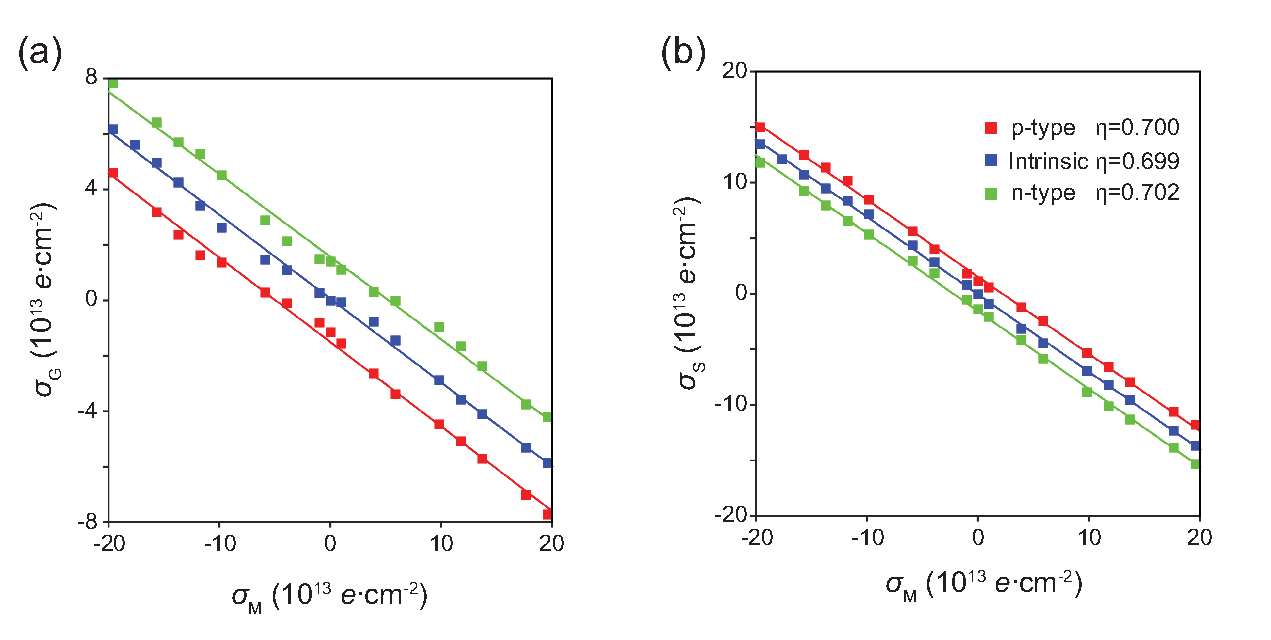
\includegraphics[width=0.95\textwidth]{img/SI-larger-sigma_M.eps}
  \caption{Induced charge densities at (a) graphene, $\sigma\subs{G}$, and (b) Si(111), $\sigma\subs{S}$, as a function of $\sigma\subs{M}$ in different systems: intrinsic (blue), p-type (green)  and n-type (red) Si, respectively.
  The doping levels of Si are the same as in Figure 4 in the main body. 
  $\sigma\subs{M}$ ranges from $-20\times10^{13}$ $e\cdot$cm$^{-2}$ to $20\times10^{13}$ $e\cdot$cm$^{-2}$. 
  The $\eta$ values are extracted by linear-fitting of the $\sigma\subs{S}-\sigma\subs{M}$ curves.}
  \label{fig:sigma-larger}
\end{figure}

\begin{figure}
  \centering
  \includegraphics[width=0.95\textwidth]{img/SI-1-DOS.eps}
  \caption{Density of states as a function of relative energy level of several selected 2D materials (MoS$\subs{2}$, MoSe$\subs{2}$, MoTe$\subs{2}$, WS$\subs{2}$, WSe$\subs{2}$, WTe$\subs{2}$, phosphorene, graphene, silicene and germanene) by HSE06 hybrid functional method.}
  \label{fig:DOS}
\end{figure}

\newpage
\section{Effect of interface States on the Transparency of Monolayer 2D Materials} 
Here we model how the interface states at the 2D material-semiconductor interface influence the performance of a MOGS QC,
including their effect on the transparency of monolayer 2D materials.
We consider a classical model which assumes the interface states are atomically thin on the semiconductor surface and are completely ionized species \cite{Sze1965, Heine1965, Sze2006Mosfets}. 
The schematic illustration for the graphene-semiconductor interface considering the interface states can be found in Figure \ref{fig:scheme-interface}.
\begin{figure}[htbp]
  \centering
  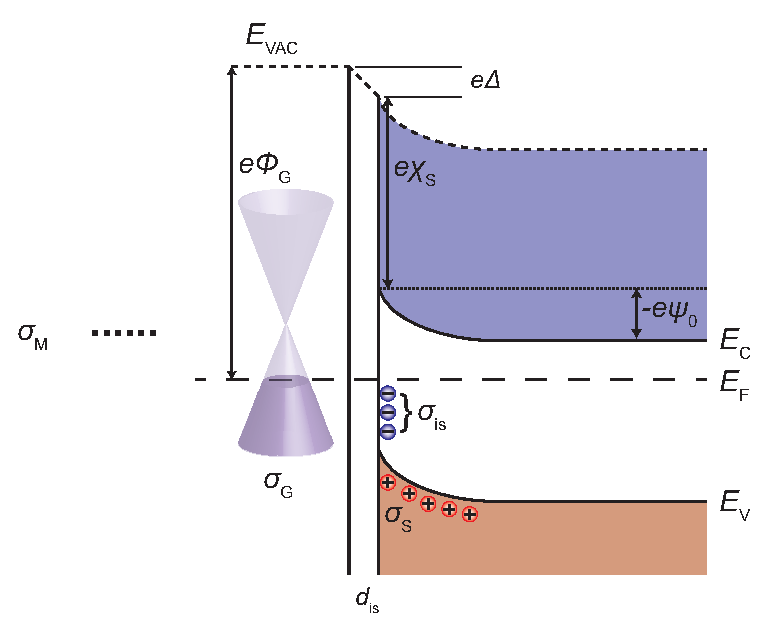
\includegraphics[width=0.65\textwidth]{img/scheme_interfacial.eps}
  \caption{Scheme for the graphene-semiconductor interface with interface states.}
  \label{fig:scheme-interface}
\end{figure}
The interface states possess a constant charge density of $\sigma\subs{is}$, which is a function of the interface density of states $D\subs{is}$ and the neutral energy level of the interface states.
The interface states create a potential drop $\Delta$ over the interface layer, which has a width of $d\subs{is}$ and permittivity $\epsilon\subs{is}$.
According to Gauss's law, $\Delta$ is dependent on both $\sigma_{is}$ and $\sigma_{S}$:
\begin{equation}
  \Delta = d\subs{is}\frac{\sigma\subs{S}+\sigma\subs{is}}{\epsilon\subs{is}}
  \label{eqn:delta_1}
\end{equation}
The potential drop results in a deviation from the Schottky-Mott rule, which is given by:
\begin{equation}
  \Delta = \frac{E_{\mathrm C,\infty} - E_{\mathrm F,\infty}}{e} + \chi\subs{S} -\psi_0 - \phi\subs{G}
  \label{eqn:delta_2}
\end{equation}
Combining eqs \ref{eqn:delta_1} and \ref{eqn:delta_2}, it follows:
\begin{equation}
  d\subs{is}\frac{\sigma\subs{S}+\sigma\subs{is}}{\epsilon\subs{is}} = 
  \frac{E_{\mathrm C,\infty} - E_{\mathrm F,\infty}}{e} + \chi\subs{S} -\psi_0 - \phi\subs{G}
  \label{eqn:schottkey_is}
\end{equation}
Following the same procedure of eq 10 in main text, the transparent index $\eta$ is given by:
\begin{equation}
  \begin{aligned}
      \eta &= -\frac{\partial \sigma\subs{S}}{\sigma\subs{M}} \\
           &= -\frac{\partial \sigma\subs{S}}{\partial \psi_0} \frac{\partial \psi_0}{\partial \phi\subs{G}} \frac{\partial \phi\subs{G}}{\sigma\subs{G}} \frac{\partial \sigma\subs{G}}{\partial \sigma\subs{M}} \\
           &= \frac{C\subs{S}}{C\subs{G}} \frac{\partial \psi_0}{\partial \phi\subs{G}}(\eta-1)\\
           &= \dfrac{1}{1 - \dfrac{C\subs{G}}{C\subs{S}}\dfrac{\partial \phi\subs{G}}{\partial \psi_0}}\\
           &= \dfrac{1}{1+k\dfrac{\partial \phi\subs{G}}{\partial \psi\subs{0}}}
  \end{aligned}
\end{equation}
Compared to eq 10 in main text, the factor $k=-\dfrac{\partial \phi\subs{G}}{\partial \psi\subs{0}}$ is given by eq \ref{eqn:schottkey_is}:

\begin{equation}
  \begin{aligned}
      k &= -\frac{d\subs{is}}{\epsilon\subs{is}}( 
            \frac{\partial \sigma\subs{is}} {\partial \psi_0} 
            + \frac{\partial \sigma\subs{S}}{\partial \psi_0} ) +1 \\
        &=  \frac{d\subs{is}}{\epsilon\subs{is}}C_{S} +1
  \end{aligned}
\end{equation}
Finally we obtain the expression for the transparency through a monolayer graphene when the interface states are considered, as follows:
\begin{equation}
  \begin{aligned}
      \eta &= \dfrac{1}{1+k\dfrac{C\subs{G}}{C\subs{S}}}\\
           &= \dfrac{1}{1+\dfrac{d\subs{is}}{\epsilon\subs{is}}C\subs{G} +\dfrac{C\subs{G}}{C\subs{S}} }\\
           &= \dfrac{1}{1+\dfrac{C\subs{G}}{C\subs{is}} +\dfrac{C\subs{G}}{C\subs{S}} }
  \end{aligned}
\end{equation}

Note that the final expression for $\eta$ is independent of $\sigma\subs{is}$. 
Instead, the governing parameter is the geometric capacitance of the interface layer $C\subs{is}=\dfrac{\epsilon\subs{is}}{d\subs{is}}$.
Accordingly, the transparency when considering the interface layer is always lower than that in the ideal case (when $d\subs{is}=0$).
On a clean semiconductor surface, $d\subs{is}$ is as low as 0.4-0.5 nm.
Since $\epsilon\subs{is}$ is larger than $\epsilon\subs{0}$, we infer that $C\subs{is}$ is comparable to $C\subs{G}$.
On the other hand, when the interface layer is thicker (e.g. long-chain hydrocarbon adsorption), $C\subs{is}$ is much lower than that on a clean semiconductor surface, thereby resulting in a lower transparency.
The above analysis would also be valid for other 2D materials (by substituting $C\subs{G}$ with the general term $C\subs{Q}$).

We would like to point out that the above model is derived under the assumption that $\sigma\subs{is}$ is constant and independent of $\sigma\subs{S}$ and $\sigma\subs{G}$, which might not be very realistic.
More experimental results are required to gain better insights at the interface.
\newpage

\section{Modeling the Penetration through Multilayer Graphene in a MOGS QC}
In this section we propose a simplified model for the penetration of an electric displacement field through multilayer graphene in a MOGS QC.
The interfacial coupling is ignored and each layer possesses the same electronic property, as schematically illustrated in Figure \ref{fig:scheme_ML_MOGS}.
\begin{figure}[htbp]
  \centering
  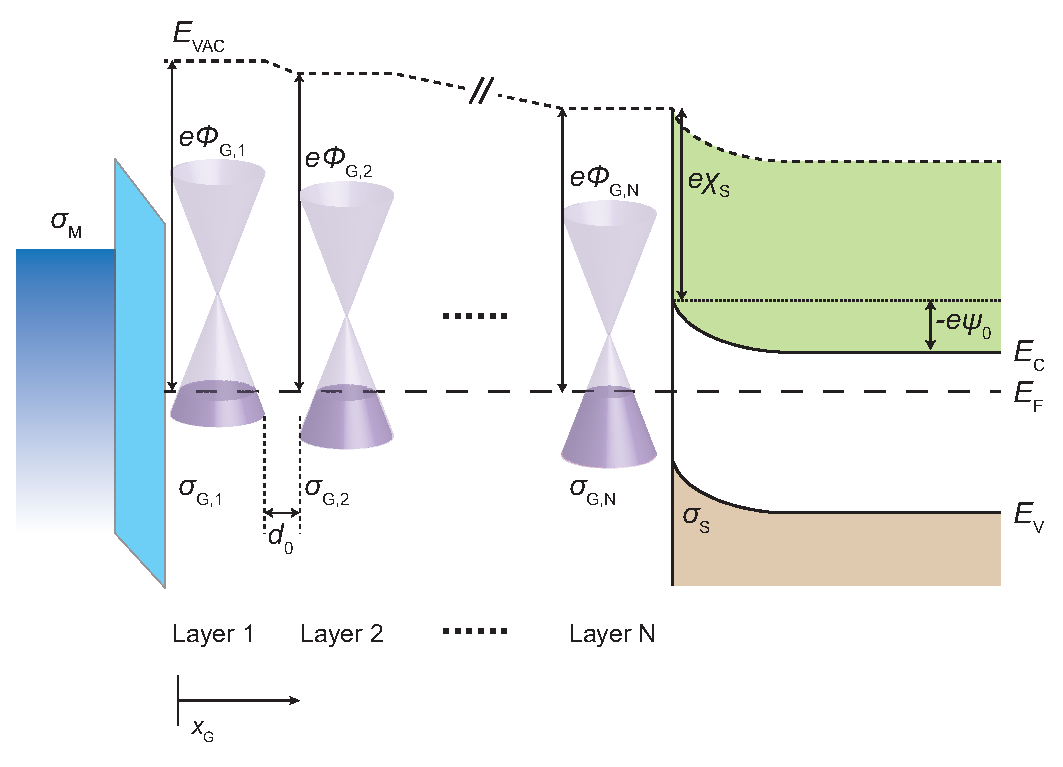
\includegraphics[width=0.95\textwidth]{img/SI_ML_graphene.eps}
  \caption{Schematic for the multilayer graphene MOGS QC system}
  \label{fig:scheme_ML_MOGS}
\end{figure}

We assume that each graphene layer is separated by a distance $d_0$ (ca. 0.33 nm) with permittivity of $\epsilon_G$ (taken the value of graphite \cite{Lui2011, Regan2012ScreeningEngineered}, $\epsilon_G\approx2.4\epsilon_0$).
We neglect the space between the first graphene layer and the oxide layer, as well as the interface states between the last graphene layer and the semiconductor layer.
The electric fields in the oxide layer and the electric field at the semiconductor surface are $\E{ox}$ and $\E{S}$, respectively.
The electric field between the $i$ and $i+1$ graphene layer is expressed as $\E{G,i}$.
Consider a multilayer graphene with layer number $N$, for the $i$-th graphene layer $\sigma\subs{G,i}$, Gauss's law suggests: 
\begin{enumerate}
  \item $i=1$\\
    \begin{equation}
      \E{ox}\epsilon\subs{ox} + \sigma\subs{G,1} - \E{G,1}\epsilon\subs{G} = 0
    \end{equation} 
  \item $i=2$$\cdots$ $N-1$\\
    \begin{equation}
      \E{G,i-1}\epsilon\subs{G} + \sigma\subs{G,i} - \E{G,i+1}\epsilon\subs{G} = 0
    \end{equation}  
  \item $i=N$\\
    \begin{equation}
      \E{G,N-1}\epsilon\subs{G} + \sigma\subs{G,N} - \E{S}\epsilon\subs{S} = 0
    \end{equation}
\end{enumerate}
Also note that the difference between the vacuum energy level $E\subs{VAC}$ between $i$ and $i+1$ graphene layers ($i=1\cdots N-1$) is identically the difference between the work function of the two layers:
\begin{equation}
  \E{G,i}d_0 = \phi\subs{G,i+1} - \phi\subs{G,i}
\end{equation}
The series of equations can therefore be solved numerically in a self-consistent approach by giving a initial value of $\E{S}$.

\begin{figure}[htbp]
  \centering
  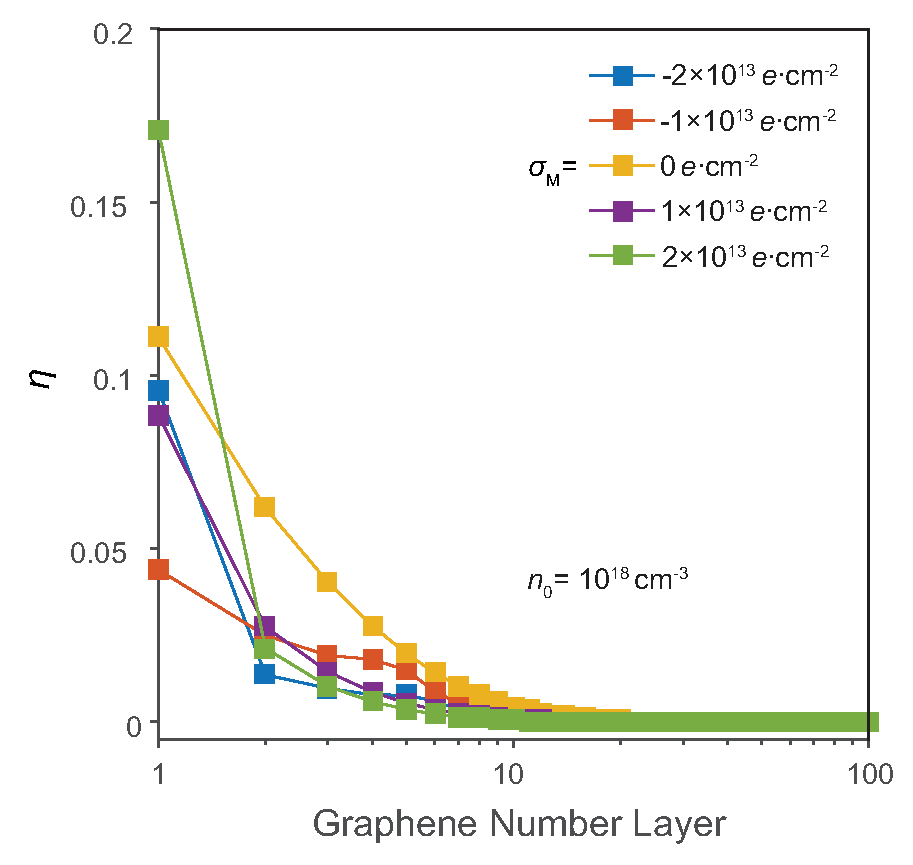
\includegraphics[width=0.75\textwidth]{img/ML_transparency_S.eps}
  \caption{Calculated transparency index $\eta$ as a function of layer number $N$, corresponding to Figure 3b in main text.}
  \label{fig:ML_trans}
\end{figure}

\begin{figure}[htbp]
  \centering
  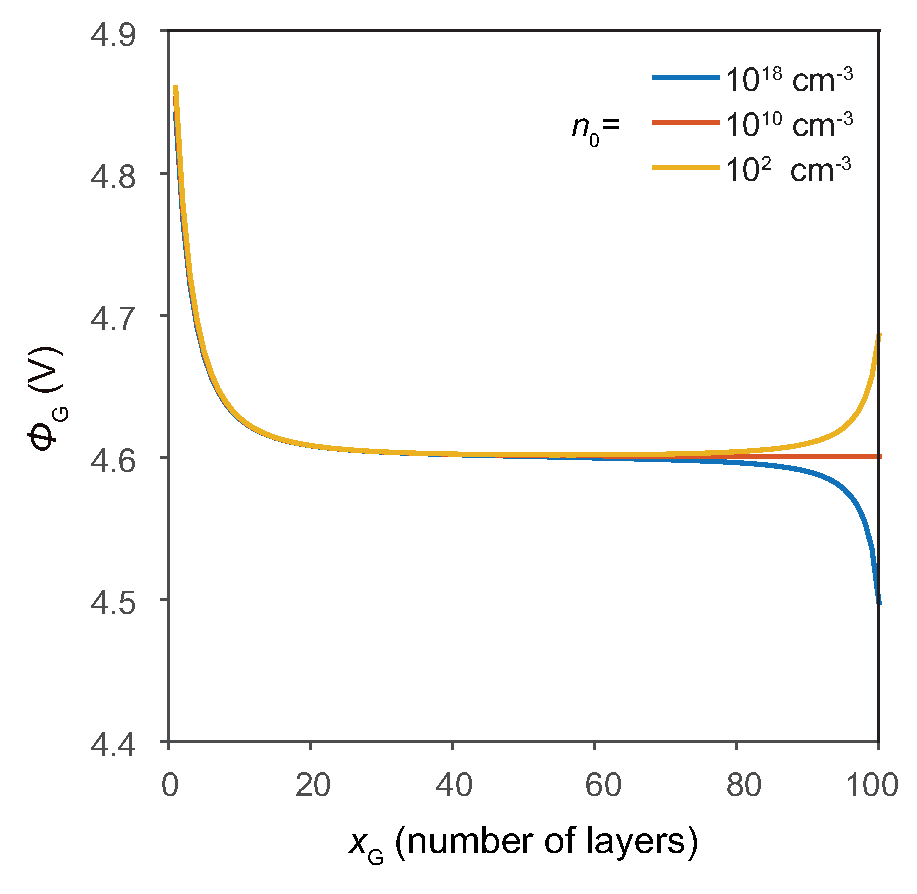
\includegraphics[width=0.75\textwidth]{img/ML_boundary.eps}
  \caption{The work function of 100-layer graphene as a function of distance from the oxide-graphene interface $x\subs{G}$ (in number of layers),
  when $\sigma\subs{M}=-10\sups{13}\ e\cdot \mathrm{cm}^{-2}$.
  Three cases are considered ($n_0=10^{18}\ \mathrm{cm}\sups{-3}$, $n_0=10^{10}\ \mathrm{cm}\sups{-3}$ and $n_0=10^{2}\ \mathrm{cm}\sups{-3}$, respectively).
  The boundary layer of graphene with oxide remains indistinguishable while the boundary layer at the graphene-semiconductor interface is determined by the doping level of semiconductor.
  Away from the boundary layers, the graphene layers remains charge neutral ($\phi_{G}=4.6\ V$).
  These results indicate that the electric field can only penetrate into a limited length in multilayer graphene.
  }
  \label{fig:ML_boundary}
\end{figure}




\newpage
\section{Band Diagrams of a MOGS QC under Different Conditions}
\begin{figure}[h!]
  \centering
  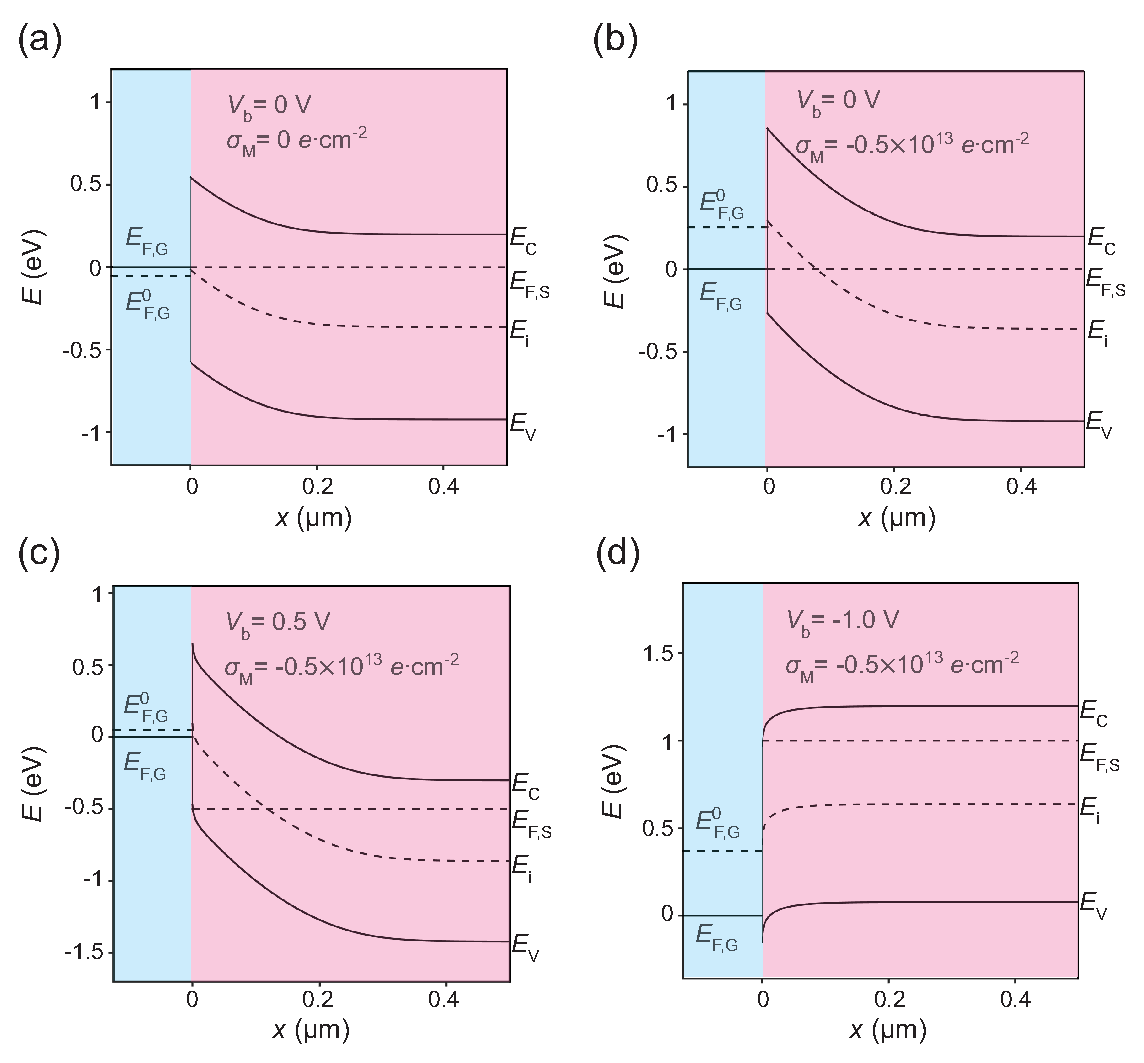
\includegraphics[width=0.95\textwidth]{img/energy_diagram.eps}
  \caption{Representative band  diagrams of the MOGS QC near the interface of graphene (blue) and semiconductor (red), under various conditions: (a) $V\subs{b}=0$ V, $\sigma\subs{M}=0$ $e\cdot$cm$\sups{-2}$; (b) $V\subs{b}=0$ V, $\sigma\subs{M}=-0.5\times10^{13}$ $e\cdot$cm$\sups{-2}$; (c) $V\subs{b}=0.5$ V, $\sigma\subs{M}=-0.5\times10^{13}$ $e\cdot$cm$\sups{-2}$; (d) $V\subs{b}=-1.0$ V, $\sigma\subs{M}=-0.5\times10^{13}$ $e\cdot$cm$\sups{-2}$. The Si layer has a doping level of 10$\sups{16}$ cm$\sups{-3}$. The $E_{\mathrm{F,G}}$ is drawn in solid line and set to 0 eV, while the Fermi level at CNP, $E_{\mathrm{F,G}}^0$ is demonstrated as dashed line.  The Fermi level   $E_{\mathrm {F,S}}$, conduction band $E\subs{C}$ ,  mid-gap $E\subs{i}$  and  valence band $E\subs{V}$ energy levels of semiconductor are displayed, respectively.}
  \label{fig:energy-diagram}
\end{figure}
To overview the macroscopic model, several representative band diagrams are drawn in Figure \ref{fig:energy-diagram} to explicate the influence of both gating and bias in a MOGS QC ($N\subs{D}=10^{16}$ cm$^{-3}$ for the Si layer).
The conduction band, valence band and mid-gap energy levels in semiconductor are described by (i) $E\subs{C}(x)=E_{\mathrm{C,\infty}}-e\psi(x)$,  (ii) $E\subs{V}(x)=E_{\mathrm{V,\infty}}-e\psi(x)$ and (iii) $E\subs{i}(x)=E_{\mathrm{i,\infty}}-e\psi(x)$, respectively, where $\psi(x)$ is solved by applying boundary conditions $\psi(0)=\psi_0$ and $\psi(\infty)=0$  for eq 3 in the main body.
In the case of free contact (Figure \ref{fig:energy-diagram}a), the deviation between graphene's Fermi level $E_{\mathrm{F,G}}$ with the CNP Fermi level $E_{\mathrm{F,G}}^0$ indicates that a small degree of charge transfer readily takes place at the SG interface. 
When a negative $\sigma\subs{M}$ of $-0.5\times10^{13}$ $e\cdot$cm$^{-2}$ is applied (Figure \ref{fig:energy-diagram}b), the $E_{\mathrm{F,G}}$ significantly shifts due to the charge induction via the field effect.
Note that the space charge at the SG interface is also tuned to weak inversion state from the depletion state at free contact, indicating the ``penetration'' of positive charge from the graphene 2DEG to the semiconductor layer. 
In Figure \ref{fig:energy-diagram}c, a reverse bias of 0.5 V is further applied in addition to Figure \ref{fig:energy-diagram}b. 
We observe that $E_{F,G}$ shifts back near the CNP of graphene, and a weak inversion layer at the SG interface is formed.
This is a clear indication that bias can interfere with the gate control by $\sigma\subs{M}$.
On the other hand, at the forward bias regime when a $V\subs{b}=-1.0$ V is applied (Figure \ref{fig:energy-diagram}d), an accumulation layer is generated at the SG interface, and the $E_{F,G}$ is observed to move away from $E_{\mathrm{F,G}}^0$ compared with Figure \ref{fig:energy-diagram}b.
Note that in the reverse bias regime, less $|V\subs{b}|$ is required to exert obvious influence over $E_{\mathrm{F,G}}$ than in the forward regime, because once the SG interface layer is weakly inverted, more bias is needed to turn the interface layer to accumulation than to strong inversion.
We conclude from energy diagrams in both reverse and forward bias regimes that applying a high $|V\subs{b}|$ will significantly dilute the effect of gating control in a MOGS QC.

\newpage
\bibliography{SI}

\end{document}
